\begin{figure}[t]
    \centering
    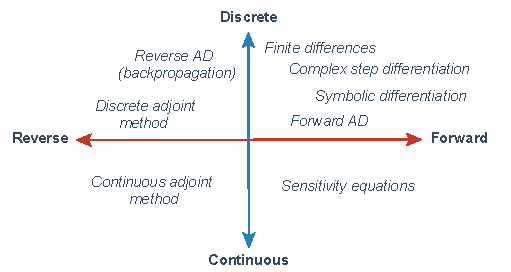
\includegraphics[width=0.80\textwidth]{figures/scheme-methods.pdf}
    \caption{Schematic representation of the different methods available for differentiation involving differential equation solutions. These can be classified depending if they find the gradient by solving a new system of differential equations (\textit{continuous}) or if instead they manipulate unit algebraic operations (\textit{discrete}). Additionally, these methods can be categorized based on their alignment with the direction of the numerical solver. If they operate in the same direction as the solver, they are referred to as \textit{forward methods}. Conversely, if they function in the opposite direction, they are known as \textit{backward methods}.}
    \label{fig:diff}
\end{figure}
Depending on the number of parameters and the complexity of the differential equation we are trying to solve, there are different methods to compute gradients with different numerical and computational advantages.
These methods can be roughly classified as:
\begin{itemize}
    \item \textit{Discrete} vs \textit{continuous} methods
    \item \textit{Forward} vs \textit{backward} methods
\end{itemize}
The first difference regards the fact that the method for computing the gradient can be either based on the manipulation of atomic operations that are easy to differentiate using the chain rule several times (discrete), in opposition to the approach of approximating the gradient as the numerical solution of a new set of differential equations (continuous).
Another way of conceptualizing this difference is by comparing them with the discretize-differentiate and differentiate-discretize approaches \cite{bradley2013pde, Onken_Ruthotto_2020, FATODE2014, Sirkes_Tziperman_1997}.   
We can either discretize the original system of ODEs in order to numerically solve it and then find an strategy to differentiate it; or instead define new equations for the differentiation step and later numerically solver them.

The second distinction is related to the fact that some methods compute gradients by resolving a new sequential problem that may move in the same direction as the original numerical solver - i.e. moving forward in time - or, instead, they solve a new system that goes backwards in time. 
Figure \ref{fig:diff} displays a classification of some methods under this two-fold classification. 
In the following section, we explore more in detail these methods.

It is important to note that if all the methods we explore in this section are mathematically correct, \textit{that does not imply they are numerically stable}.
These statements applied to methods based on pure automatic differentiation as well as adjoint methods. 
We explore this consideration in more detail in section \ref{sec:computational-implementation}.
